\subsection{sCenario and gOal based SysteM develOpment methoD (COSMOD) (FDD)}\label{scgo}
COSMOD-Requirements Engineering (COSMOD-RE) beschreibt ein iteratives Vorgehen zum gleichzeitigen Design von Anforderungen und Software-Architektur. Kerngedanke bei COSMOD-RE ist eine Aufteilung in vier Hierarchiestufen, wo sowohl Architektur als auch Anforderungen definiert werden. In diesen vier Hierarchiestufen wird einerseits aus der Anforderungssicht und andererseits aus der Architektursicht betrachtet, welche Anforderungen und Komponenten dem System zuzuordnen sind.\\

\subsubsection{Ziele der Methode}
Kernziel von COSMOD-RE ist es die Entwicklung von Anforderungs- und Architekturartefakten f\"ur softwareintensive eingebettete Systeme zu unterst\"utzen. Ein Ziel- und Szenario-basierter Ansatz wie COSMOD-RE, der das Co-Design von Architekturartefakten und Anforderungen erm\"oglicht muss jedoch einige Anforderungen erf\"ullen um einen Nutzen zu haben. Die Anforderungen an eine solchen Methodik sind \cite{Poh02}\\
 
\begin{itemize}
\item \emph{Entwicklung von Anforderungen und Architekturartefakten.} \\
Da Anforderungen und die Software Architektur die Kerntreiber hinter innovativen Projekten sind ist es wichtig beide gleicherma\ss{}en zu nutzen, sodass keines von beiden in den Vordergrund tritt \cite{Poh02}.
\item \emph{Unterst\"utzung der Anordnung von Anforderungen und Architekturartefakten.} \\
Werden Anforderungen und Architekturartefakte parallel entwickelt kann es passieren, dass Inkonsistenzen auftreten. Um diese zu vermeiden ist es notwendig, dass COSMOD-RE diese erkennt und behebt \cite{Poh02}.
\item \emph{Definition detaillierter Anforderungen auf der Basis von Architekturartefakten.} \\
Ohne technisches Wissen f\"allt es Stakeholdern schwer notwendige Details f\"ur die Erhebung architekturrelevanter Anforderungen zu liefern. Daher sollte es COSMOD-RE erm\"oglichen die detaillierten Anforderungen erst nach der initialen Definition von Architekturartefakten zu liefern \cite{Poh02}. 
\item \emph{Nutzung einer Abstraktionshierarchie.} \\
Da bei einem Co-Design Vorgehen eine gro\ss{}e Komplexit\"at bestehen kann ist es notwendig eine Abstraktionshierarchie einzuf\"uhren um diese entsprechend zu behandeln \cite{Poh02}.\\
\end{itemize}

Ferner basieren die in der Methode genutzten Prozesse auf folgenden Ideen: \cite{Poh01} \\

\begin{itemize}
\item Initiale Unterteilung in die Architektursicht und die Systemnutzungs-Sicht
\item Szenario- und Ziel-basierte Integration der Sichtweisen
\item Definition von Systemanforderungen basierend auf einer festgelegten Systemnutzungs- und Architektur-Sicht \\
\end{itemize}

\subsubsection{Funktionsweise der Methode}
Das wichtigste Element von COSMOD-RE ist die Abstraktionshierarchie. \"Uber diese werden alle Aktivit\"aten, die im Rahmen der Methodik stattfinden, eingeordnet und miteinander in einen Kontext gesetzt. So wird auf jeder Ebene der Abstraktionshierarchie eine Architektursicht und eine Anforderungssicht erzeugt. Hierbei ist jedoch zu beachten, dass bei COSMOD-RE nicht unbedingt ein Top-Down-Ansatz zu w\"ahlen ist, da Anforderungsartefakte und Architekturartefakte auf allen Ebenen gleichzeitig bearbeitet werden k\"onnen.\\

\begin{figure}[h]
	\centering
	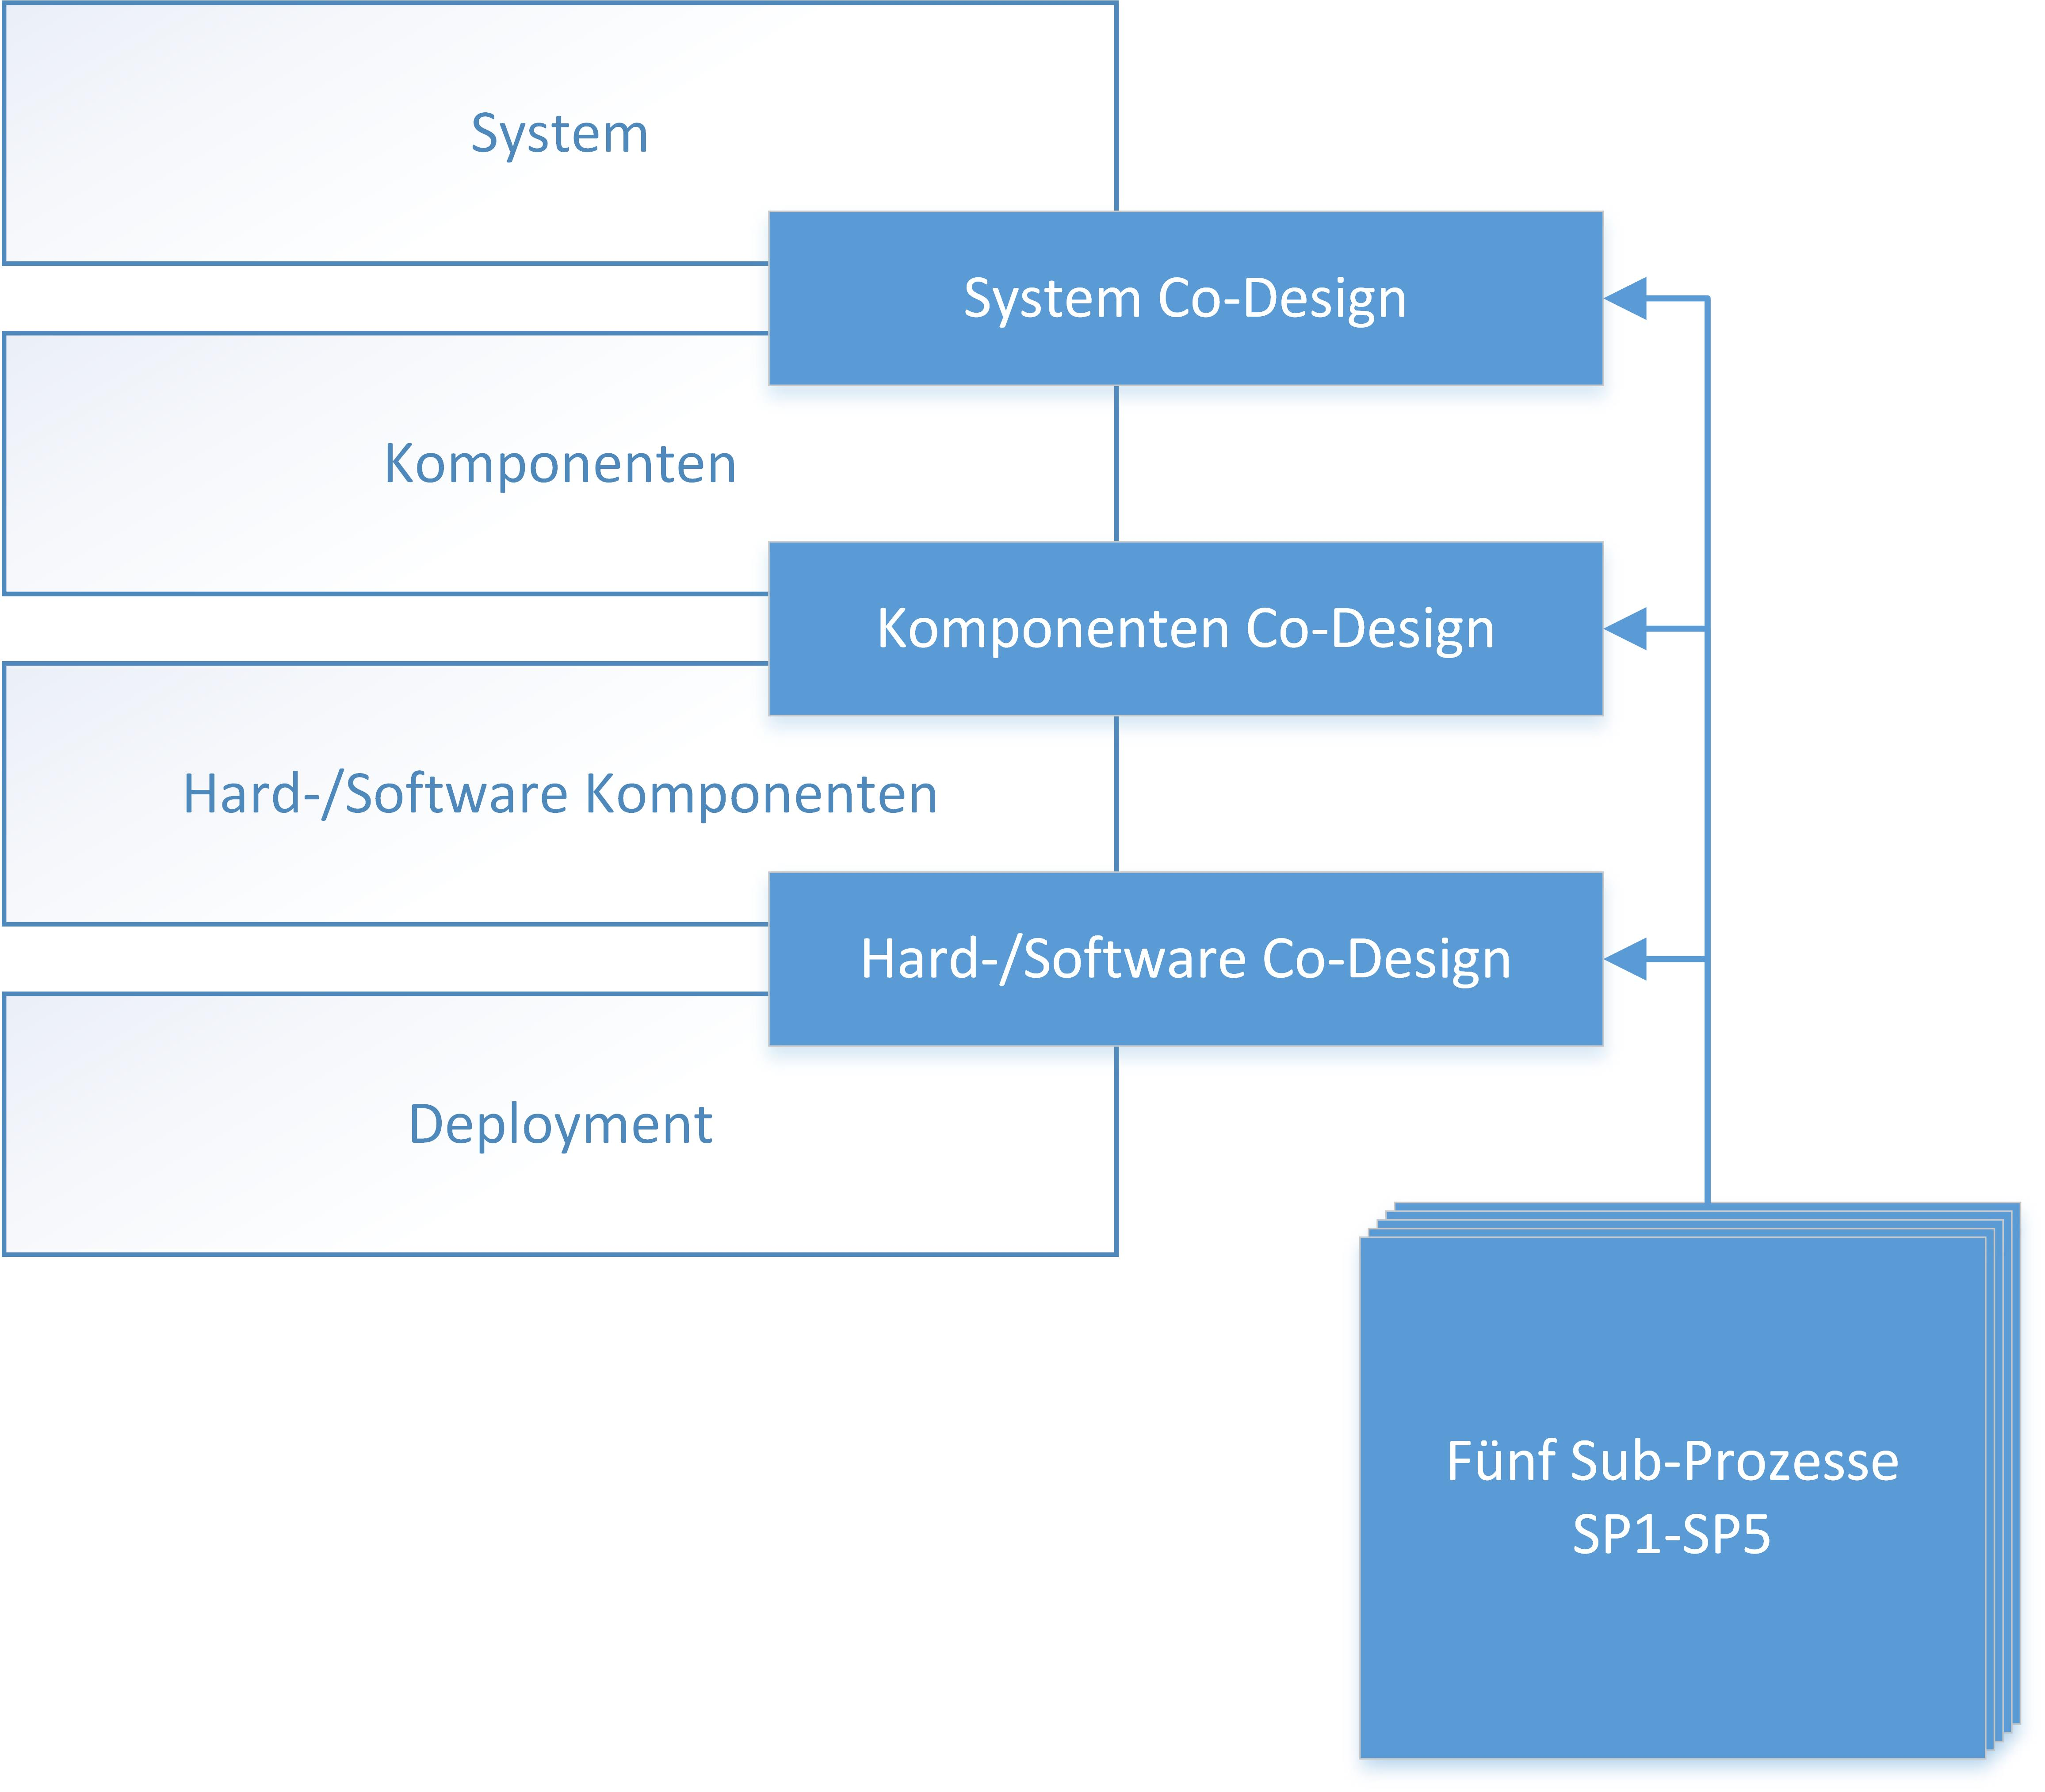
\includegraphics[scale=0.75]{COSMODREoverview.jpg} 
	\caption{Schematische Darstellung der COSMOD-RE Methode}\label{cosmodreow}
\end{figure}

In der Abbildung \ref{cosmodreow} ist schematisch dargestellt wie COSMOD-RE auszuf\"uhren ist. Es gibt vier Hierarchieebenen, auf denen drei Co-Design Prozesse arbeiten, die wiederum aus f\"unf Subprozessen bestehen.\\

\paragraph{Randbedingungen}
Bei der Anwendung von COSMOD-RE ist zu beachten, dass einige Bedingungen erf\"ullt sein m\"ussen um die Methodik richtig anzuwenden:\\

\begin{itemize}
\item \emph{Definition einer Abstraktionshierarchie.} \\
Es gibt keine Richtlinien bez\"uglich der Definition der Abstraktionshierarchie. Dies bedeutet, dass die verwendeten Hierarchiestufen in jedem Projekt neu festgelegt werden m\"ussen. Ferner ist hierbei von Relevanz, zu definieren, wo die Trennlinien zwischen verschiedenen Abstraktionsstufen sind \cite{Sik01}.
\item \emph{Verkn\"upfung von Anforderungs- und Architekturmodellen.} \\
Da im Rahmen von COSMOD-RE Anforderungsartefakte und Architekturartefakte parallel entwickelt werden ist es notwendig diese miteinander zu verkn\"upfen, um sie in den Kontext des Ziels der Software zu bringen. F\"ur diese Verkn\"upfung ist die Anwendung von Methodenfragmenten notwendig \cite{Sik01}.
\item \emph{Definition von Konsistenzbedingungen.} \\
F\"ur die Definition von Konsistenzbedingungen gibt es keinen allgemeing\"ultigen Ansatz. Daher ist es notwendig in jedem Projekt neu zu definieren, ob Konsistenz gegeben ist oder nicht \cite{Sik01}.
\item \emph{Definition der System-Vision.} \\
Es muss eine System-Vision vorhanden sein um COSMOD-RE einsetzen zu k\"onnen, da die Methode diese zu Anforderungen verfeinert \cite{Poh01}.\\
\end{itemize}

Sind diese Randbedingungen gekl\"art ist es m\"oglich COSMOD-RE anzuwenden.\\

\paragraph{Eingabe}
Als Eingabe ben\"otigt COSMOD-RE eine System-Vision. Dies bedeutet, in initialen Gespr\"achen mit Stakeholdern muss bereits festgehalten sein, welche Vision von dem zu konzipierenden System gegeben ist. Die System-Vision ist vor allem in der Systemebene von Relevanz. auf den niedrigeren Ebenen sind die Ausgaben der oberen Ebenen bedeutsam.\\

\paragraph{Vorgehensmodell}
Um das Vorgehensmodell zu beschreiben muss zun\"achst gekl\"art werden, was unter den vier Hierarchieebenen zu verstehen ist. Danach werden die drei Co-Design Prozesse erl\"autert. Darauf folgt dann die Erl\"auterung der f\"unf Sub-Prozesse.\\

Die vier in Abbildung \ref{cosmodreow} dargestellten Hierarchieebenen sind:\\

\begin{itemize}
\item[1.] \emph{System:} Die Systemebene beschreibt die oberste Ebene, bei der in der Anforderungssicht das System als ganzes betrachtet wird. Im Fokus stehen dabei die Interaktionen mit dem System. Weiter werden funktionale Anforderungen und Qualit\"atsanforderungen erstellt, die sich auf das Gesamtsystem beziehen. Die Architektursicht konzentriert sich hier auf die Definition von externen Systemschnittstellen. Hier definierte Artefakte sollen prim\"ar die Kommunikation mit Stakeholdern unterst\"utzen.
\item[2.] \emph{Komponenten:} Die Komponentenebene bezeichnet die Aufteilung des Systems in einzelne Komponenten aus denen sich dieses zusammensetzen soll. F\"ur jede Komponente werden funktionale Anforderungen und Qualit\"atsanforderungen formuliert. Da in dieser Ebene die Basis f\"ur die Systemarchtitektur gelegt wird, hat die Kommunikation zwischen dem Software-Architekten und dem Requirements Engineer von besonderer Bedeutung. 
\item[3.] \emph{Hard-/Software Komponenten:} Auf dieser Ebene werden die zuvor erstellten Komponenten in Hard- und Software Komponenten aufgeteilt und weiter verfeinert. Anforderungen auf dieser Ebene sind somit speziell auf die Komponentenart bezogen. 
\item[4.] \emph{Deployment:} Auf dieser Ebene werden Softwarekomponenten programmierbaren Hardwarekomponeten zugeordnet. Anforderungen auf dieser Ebene beziehen sich auf das Deployment der Softwarekomponenten und ihrem Einfluss auf vorher definierte Anforderungen. 
\end{itemize}
Da die Zusammenarbeit zwischen Software-Architekt und Requirements Engineer vor allem in den obersten beiden Ebenen von Relevanz ist, sind die unteren beiden Ebenen in diesem Kontext zu vernachl\"assigen.\\

Ein Vorteil von COSMOD-RE ist unter anderem, dass Beziehung die sich \"uber mehrere Hierarchieebenen erstrecken, nicht vernachl\"assigt werden. Dies ist durch die CO-Design Prozesse m\"oglich. Diese geben an, dass bei der Ausf\"uhrung der Subprozesse mehrere Hierarchieebenen zu ber\"ucksichtigen sind. So wird beim System-Co-Design sowohl die Systemebene als auch die Komponentenebene betrachtet. Bei dem Komponenten Co-Design wird die Komponentenebene und diie Hard-/Software Komponentenebene betrachtet. Im Hard-/Software Co-Design wird die Hard-/Software Komponentenebene und die Deployment ebene ber\"ucksichtigt \cite{Poh02}. Jeder dieser drei CO-Design Prozesse f\"uhrt dann die f\"unf Subprozesse aus.\\ 

Das grunds\"atzliche Vorgehen von COSMOD-RE ist, dass eine Systemvision unter der Verwendung von Szenarien und Zielen zu einer Menge von Systemartefakten verfeinert wird \cite{Poh01}. Hierf\"ur nutzt die Methode f\"unf Subprozesse. \\

In Abbildung \ref{pro5} nach \cite{Poh01} sind diese zu sehen. \\

\begin{figure}[h]
	\centering
	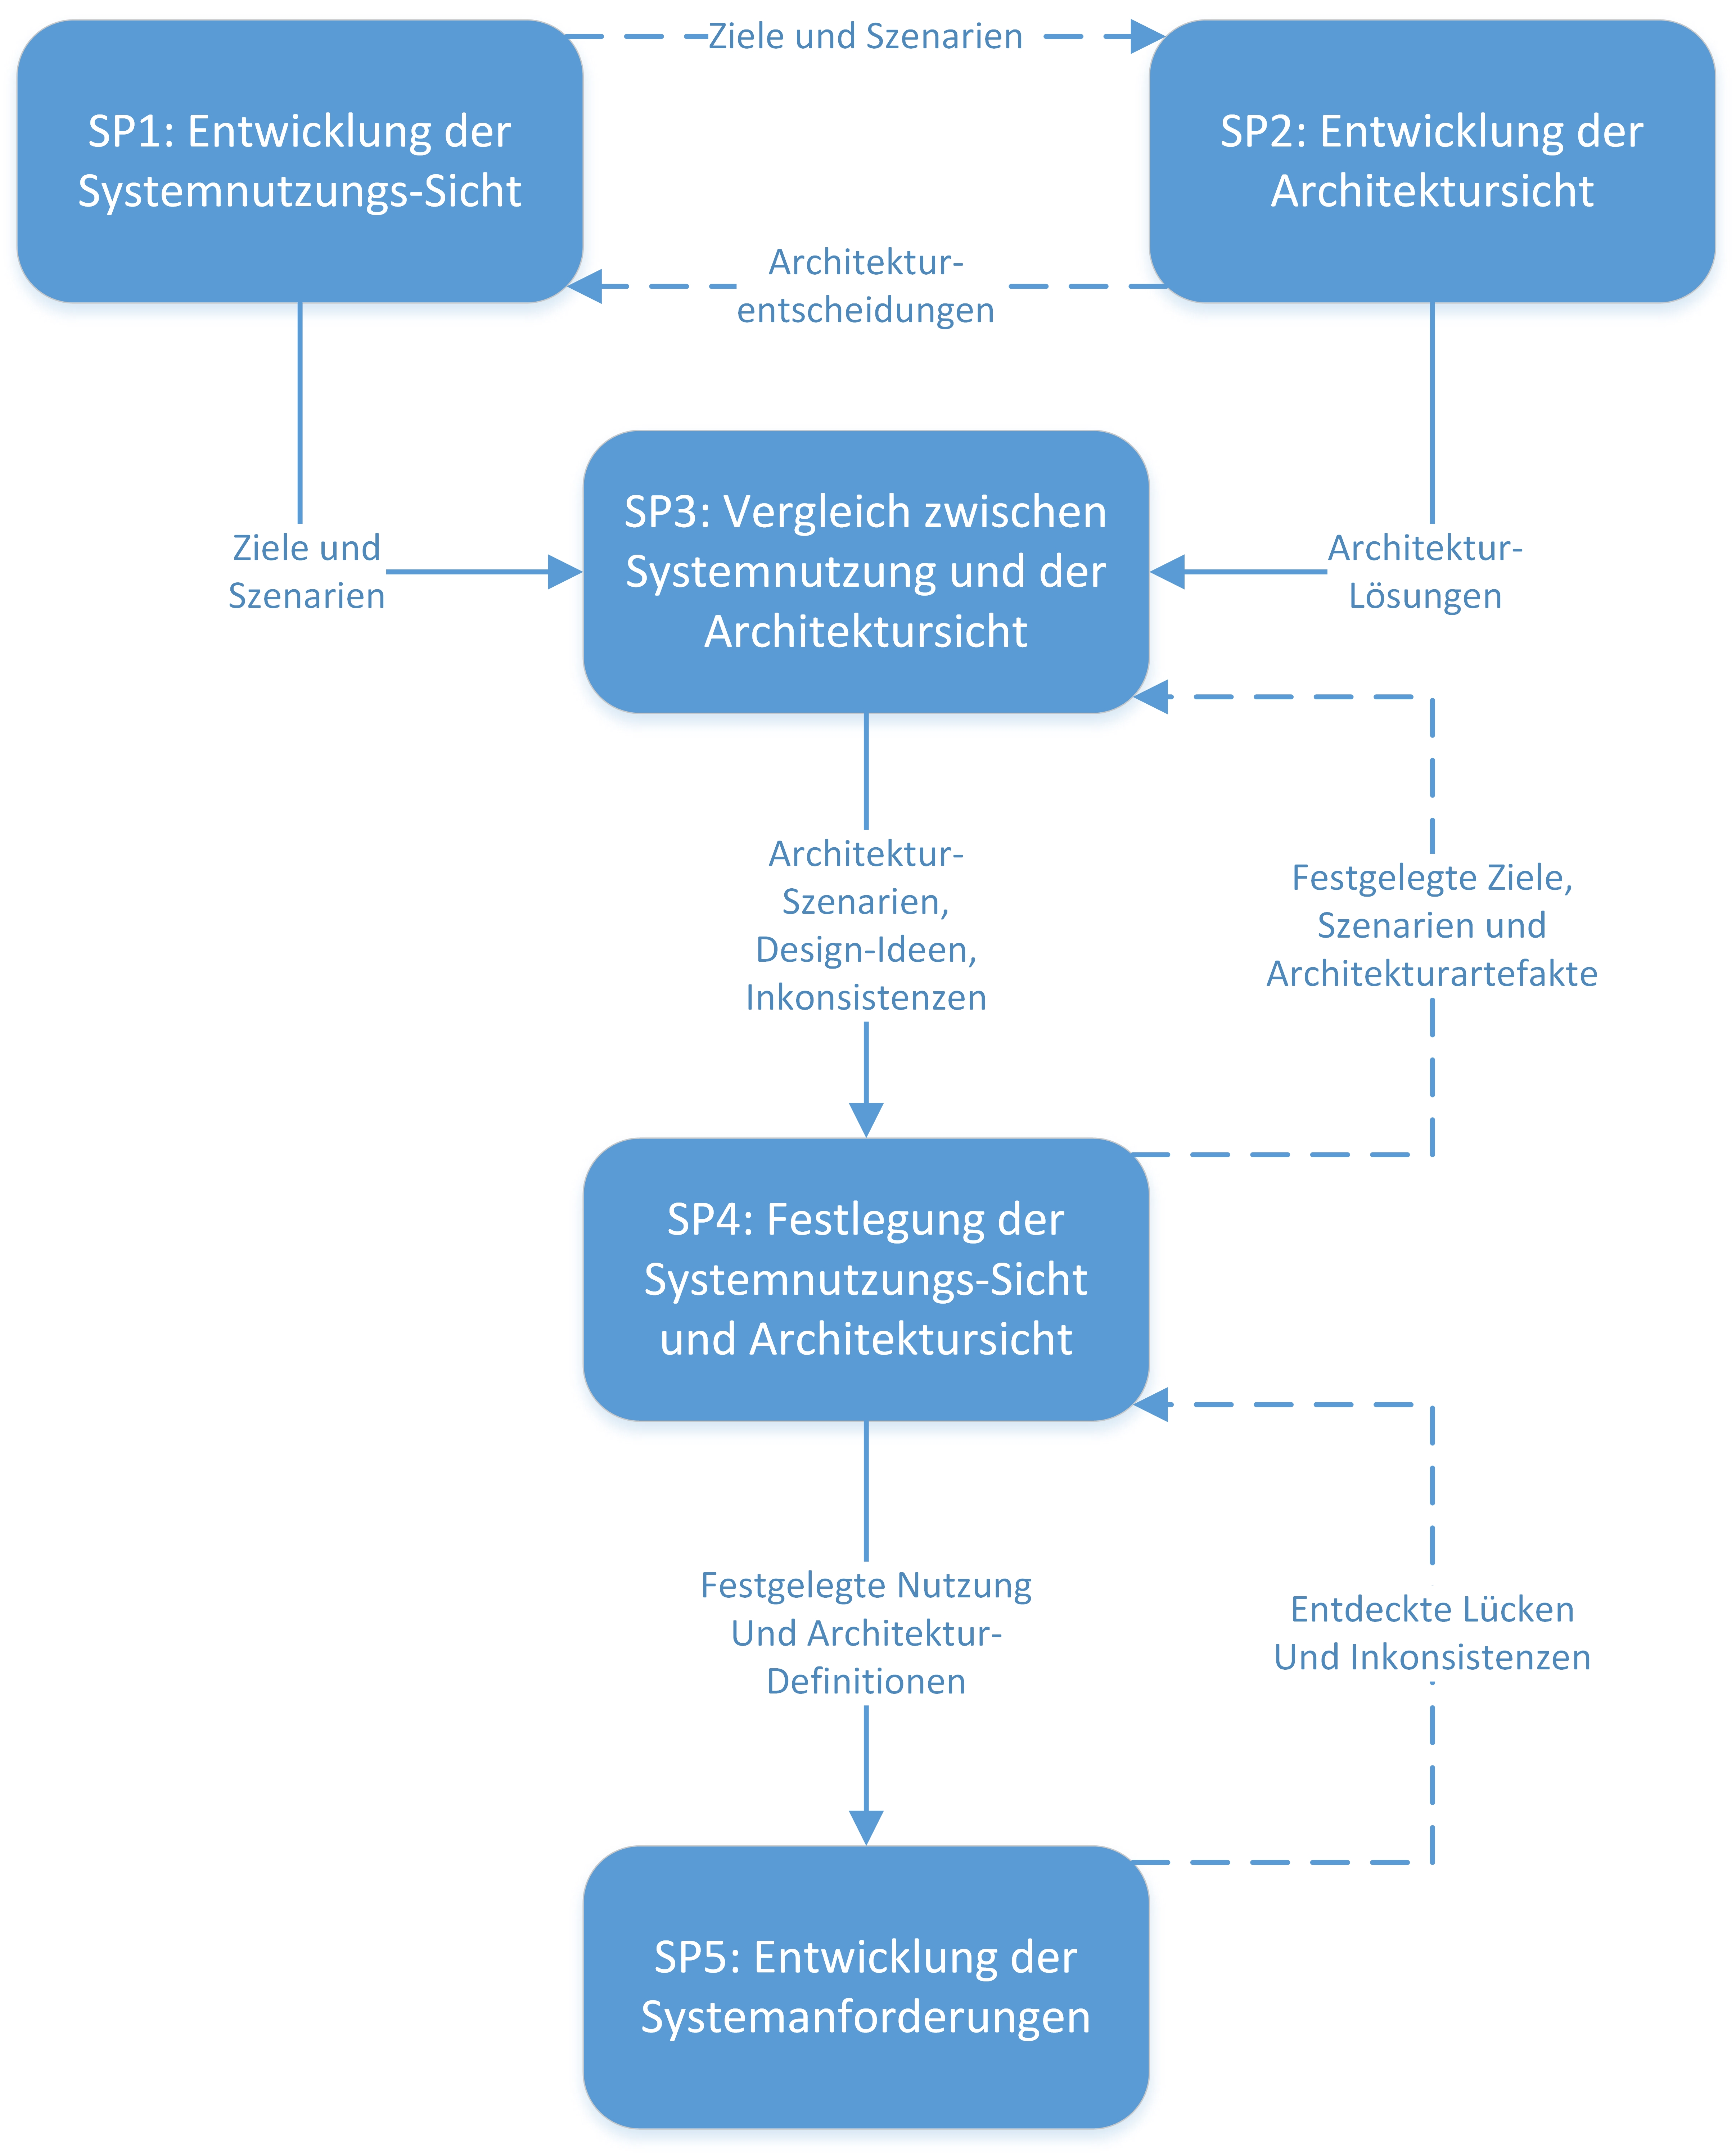
\includegraphics[scale=0.65]{COSMODRE5prozesse.jpg} 
	\caption{Die f\"unf Subprozesse der COSMOD-RE Methode}\label{pro5}
\end{figure}

\emph{SP1: Entwicklung der Systemnutzungs-Sicht -}
Ziel dieses Subprozesses ist die Verfeinerung der System Vision. Zun\"achst sollen hier potenzielle Akteure identifiziert werden. Daraufhin wird die System Vision in nutzerbezogene Unterziele aufgeteilt. Danach soll f\"ur jedes Ziel ein Nutzungs-Szenario gebildet werden, welches die Bedingungen f\"ur die Zielerreichung dokumentiert. In diesem Schritt ist als Eingabe die Eingabe der Methode, die System Vision, gegeben \cite{Poh01}. Bei diesem Prozess sind vor allem das Know-How des Requirements Engineer von Bedeutung. Dieser muss in Kooperation mit dem Kunden die Ziele dieses Subprozesses erreichen.\\

\emph{SP2: Entwicklung der Architektursicht -}
Hauptziel dieses Subprozesses ist die Erzeugung grober Architekturl\"osungen f\"ur das geplante System. Eingabe in diesem Subprozess ist einerseits wieder die System Vision, andererseits jedoch die in SP1 gebildeten Systemnutzungs-Ziele und -Szenarien. Ausgabe dieses Prozesses ist ein grober Entwurf der Systemarchitektur \cite{Poh01}.\\

In diesem Subprozess werden vier Kernaktivit\"aten ausgef\"uhrt:\\

\begin{itemize}
\item \emph{Analyse der Systemziele und Nutzungs-Szenarien:} Ziel dieser Aktivit\"at ist die Identifikation architekturrelevanter Aussagen in den Systemnutzungs-Zielen und Systemnutzungs-Szenarien. Diese k\"onnen zum Beispiel hinweise auf spezielle Komponenten sein. 
\item \emph{Kreative Entwicklung neuer Architekturl\"osungen:} Ziel dieser Aktivit\"at ist es innovative L\"osungen f\"ur das System zu erarbeiten. Auch wenn die in SP1 erzeugten Ausgaben von Bedeutung sind, ist hier vor allem das Know-How der Software-Architekten von Relevanz. Das technisches Hintergrundwissen und der Einfallsreichtum sind von zentraler Bedeutung.
\item \emph{Bewertung der entwickelten Architekturl\"osungen:} Ziel dieser Aktivit\"at ist die Auswertung der entwickelten L\"osungsans\"atze um so die besten auszuw\"ahlen. 
\item \emph{Definition einer vorl\"aufigen groben Architektur:} Ziel dieser Aktivit\"at ist die Erzeugung einer (partiellen) L\"osung basierend auf der zuvor ausgef\"uhrten Bewertung \cite{Poh01}.\\
\end{itemize} 

\emph{SP3: Vergleich zwischen Systemnutzungs-Sicht und Architektursicht -}
Hauptziel dieses Subprozesses ist einerseits die \"Uberpr\"ufung, ob die Architektur die identifizierten Systemnutzungs-Ziele und Szenarien unterst\"utzt und andererseits die Identifikation neuer Verwendungszwecke basierend auf der aktuellen groben System-Architektur \cite{Poh01}.\\

Die \"Uberpr\"ufung l\"asst sich auch betrachten als Vergleich der Ergebnisse von SP1 und SP2. Um die Systemnutzungs-Szenarien mit der Architektur zu vergleichen ist es notwendig die Systemnutzungs-Szenarien zu Architektur-Szenarien zu verfeinern. Diese Verfeinerung, die auch mithilfe von Message-Sequence-Charts durchgef\"uhrt werden kann, wird \"ublicherweise \"uber drei Schritte durchgef\"uhrt \cite{Poh01}.\\

\begin{itemize}
\item Das System wird in eine Untermenge funktionaler Anforderungen verfeinert, welche in der groben Architektur definiert werden.
\item Jeder Systemnutzung wird eine funktionale Komponente zugeordnet, die verantwortlich f\"ur die Realisierung der Interaktion mit externen Akteuren ist. 
\item System interne Interaktionen, die externe Interaktionen erm\"oglichen, werden definiert \cite{Poh01}.\\
\end{itemize}

\emph{SP4: Festlegung der Systemnutzungs-Sicht und Architektursicht -}
Wie auch in SP3 gibt es hier zwei zentrale Ziele. Einerseits sollen die in SP1 erzeugten Systemnutzungs-Ziele und -Szenarien mithilfe der Erkenntnisse aus SP3 verbessert und angepasst werden und andererseits soll die in SP2 gebildete grobe Architektur mithilfe der Erkenntnisse aus SP3 verbessert und angepasst werden \cite{Poh01}.\\

Hierf\"ur muss zun\"achst bei den Ausgaben von SP3 \"uberpr\"uft werden, ob sie zur Verbesserung der Ergebnisse von SP1 und SP2 geeignet sind. Hierf\"ur ist es angemessen ein System zur Kategorisierung einzuf\"uhren, \"uber das entschieden werden kann ob eine Verbesserung notwendig oder nicht notwendig ist. Danach werden die Ergebnisse von SP3 priorisiert. Hier wird \"uberpr\"uft welche Verbesserung zuerst umgesetzt werden sollte und welche nicht direkt notwendig sind. Zuletzt werden die Verbesserungen umgesetzt. Hier ist jedoch zu beachten, dass Verbesserungen neue Ideen hervorrufen k\"onnten oder Inkonsistenzen erzeugen k\"onnten. Daher kann es notwendig sein SP3 zu wiederholen. Diese Iteration ist solange durchzuf\"uhren, bis die Ergebnisse angemessen angeordnet und stabil sind \cite{Poh01}.\\

\emph{SP5: Entwicklung der Systemanforderungen -}
Hauptziel dieses Subprozesses ist die Spezifikation detaillierter Systemanforderungen. Grundlage f\"ur die Spezifikation sind die Systemnutzungs-Sicht und die Architektursicht. Mithilfe von Zielen, Szenarien und dem groben Architekturentwurf ist es m\"oglich detaillierte Anforderungen zu formulieren und in der Spezifikation aufzuf\"uhren.\\

\paragraph{Ausgabe}
Ausgabe der Methode ist eine kompakte Menge von System-Nutzung-Zielen, System-Interaktions-Szenarien und grobe Architekturartefakte. Ferner wird eine detaillierte System-Anforderungsspezifikation generiert.\\

Vor allem im Rahmen der f\"unf Subprozesse werden folgende Artefakte generiert:\\

\begin{figure}[h]
	\centering
	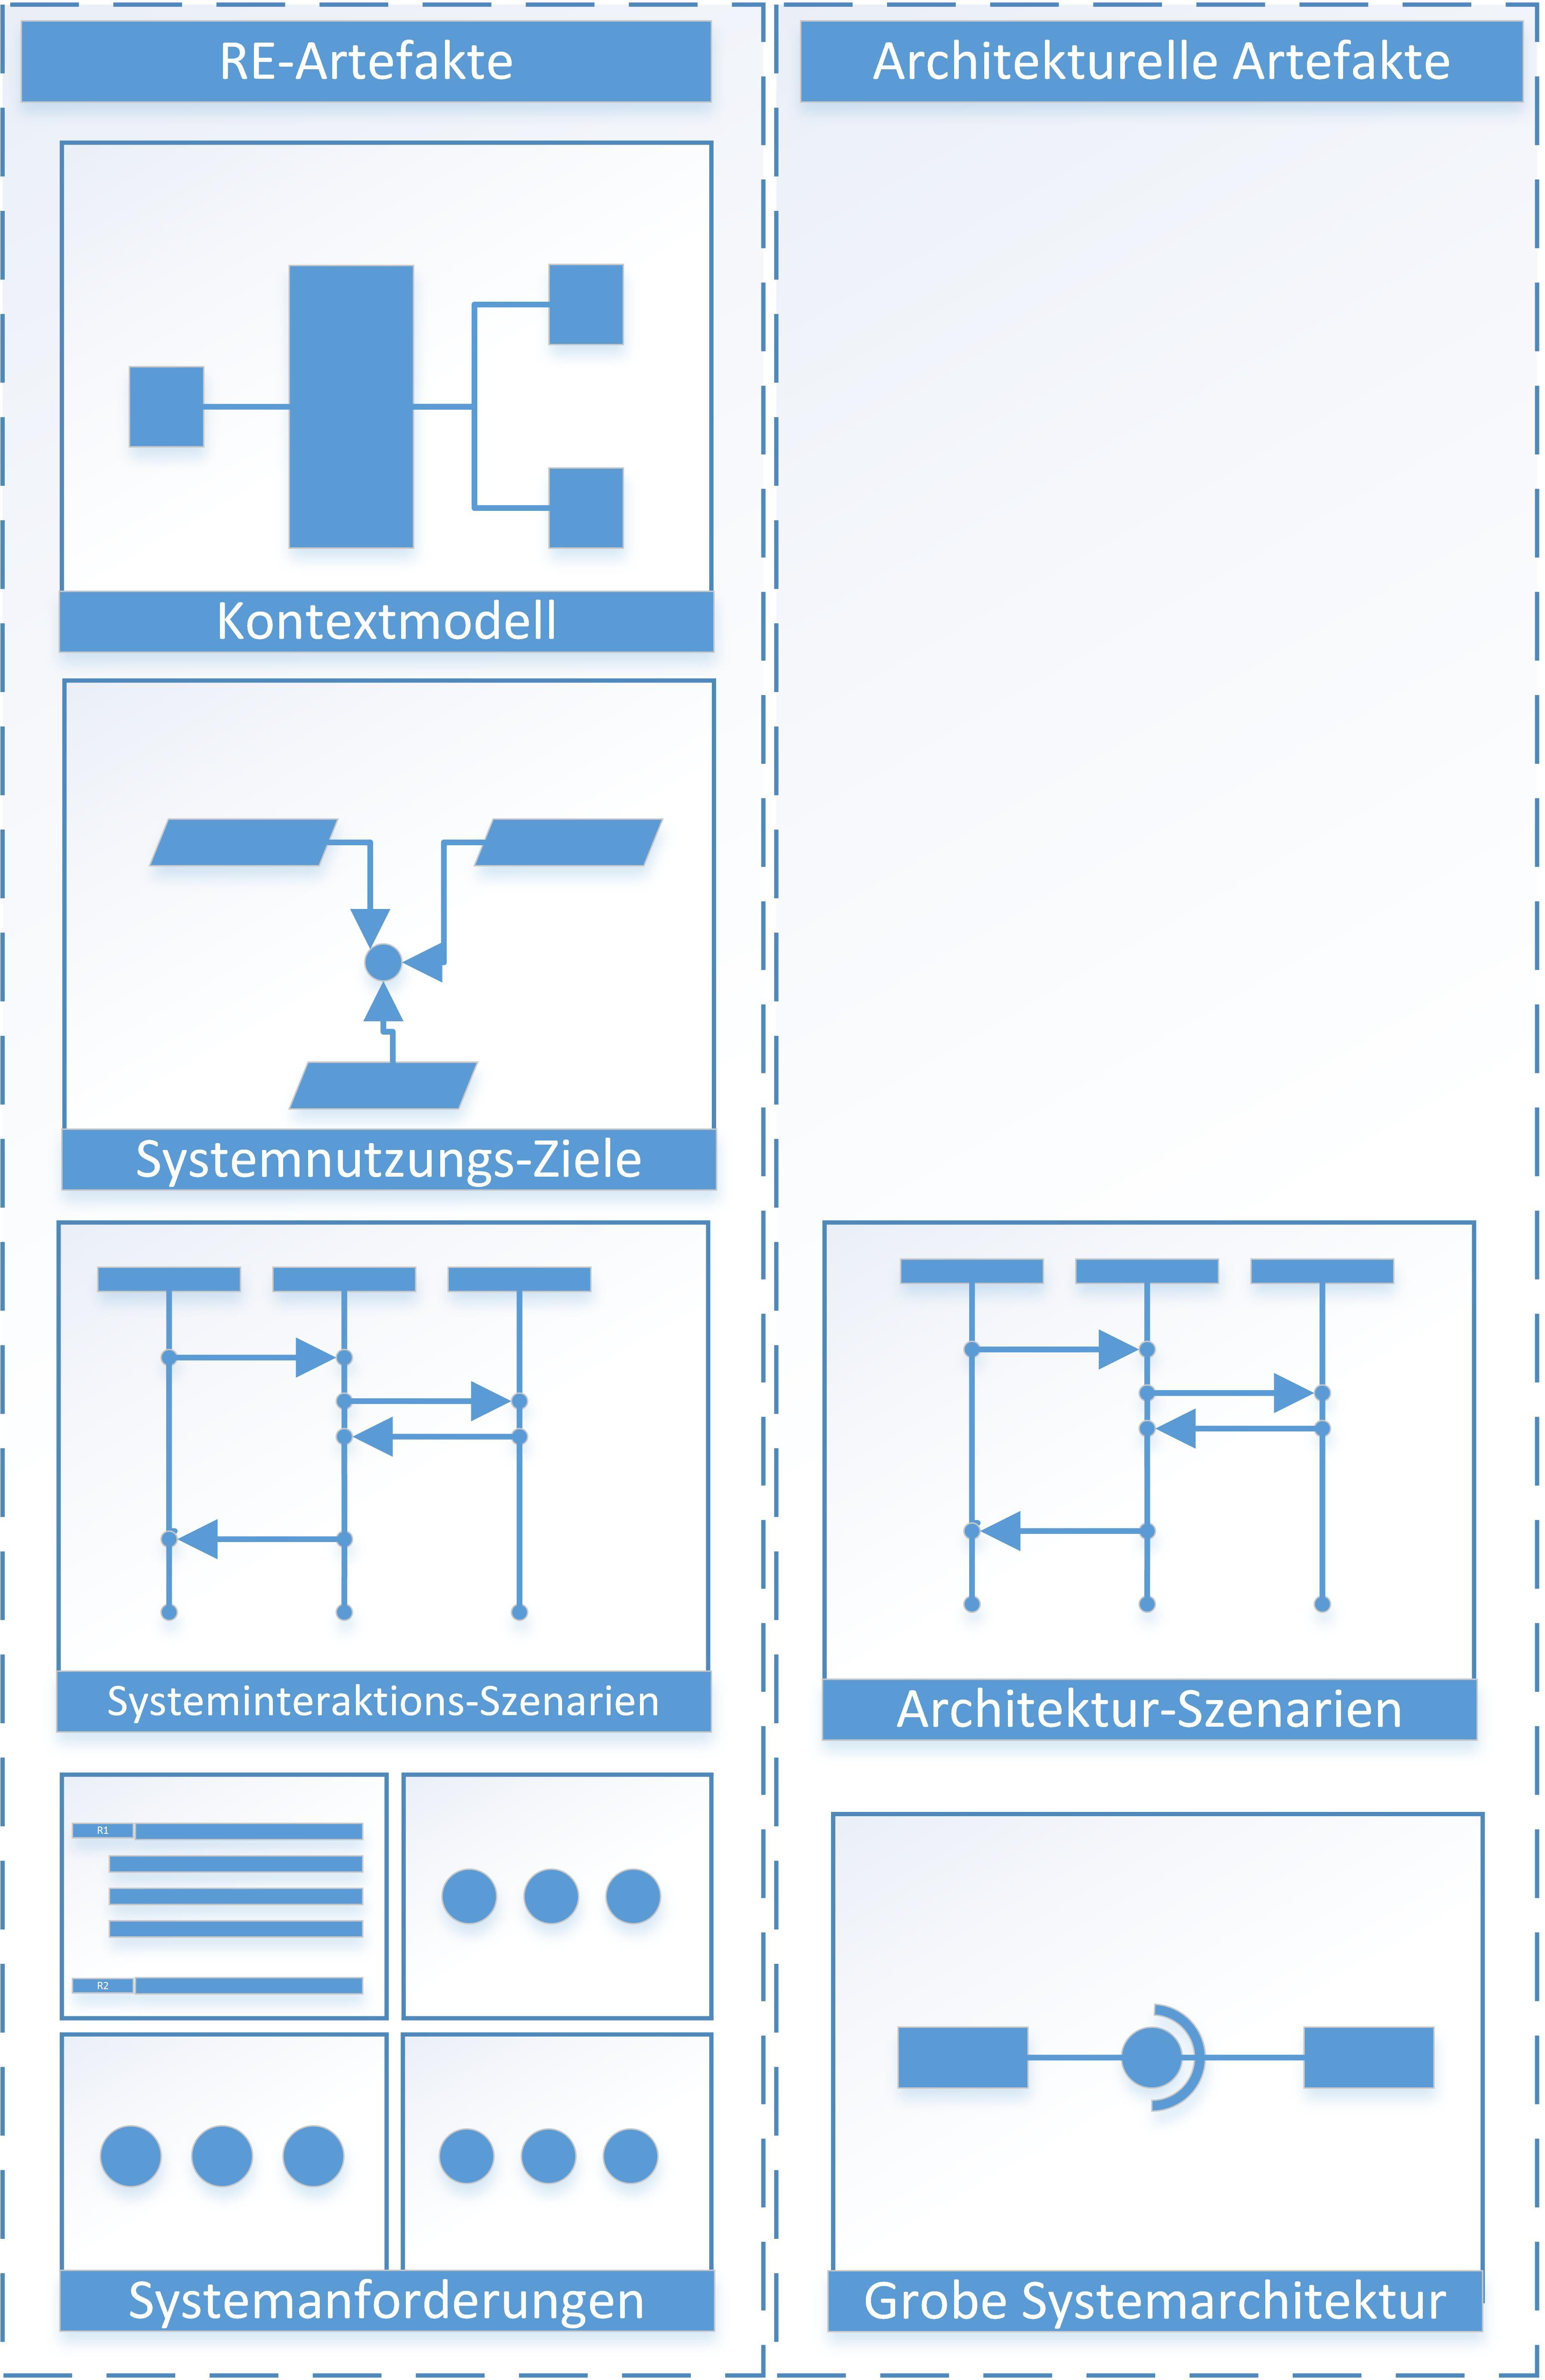
\includegraphics[scale=0.8]{artefakte.jpg} 
	\caption{Die Artefakte der COSMOD-RE Methode}\label{art}
\end{figure}

\begin{itemize}
\item \emph{Kontextmodell:}
Das Kontextmodell dokumentiert die beabsichtigte Einbettung des Systems in seine Systemumgebung. Es werden externe Akteure definiert, die mit dem System interagieren. Ein Akteur kann hierbei ein Mensch oder ein System sein. Ferner wird modelliert, wie Akteure mit dem System interagieren \cite{Poh01}.
\item \emph{Systemnutzungs-Ziele:}
Systemnutzungs-Ziele verfeiner die Systemvision. Ein Systemnutzungs-Ziel dokumentiert eine Eigenschaft des Systems in Bezug zu externen Akteuren, die das System nutzen. Ein Ziel kann hierbei in Unterziele unterteilt werden wodurch eine Hierarchie von Zielen m\"oglich ist \cite{Poh01}.  
\item \emph{Systeminteraktions-Szenarien:}
Mit diesen Szenarien werden Interaktionen von Akteuuren mit dem System dokumentiert. F\"ur die Dokumentation solcher Szenarien bieten sich modellbasierte Ans\"atze an \cite{Poh01}.
\item \emph{Architektur-Szenarien:}
Mithilfe dieser Szenarien werden Interaktionen innerhalb des Systems dokumentiert. Hiermit sind vor allem Interaktionen zwischen Systemkomponenten gemeint \cite{Poh01}. 
\item \emph{Grobe System-Architektur:}
Hier wird eine Zerlegung der System-Architektur in eine Menge funktionaler Komponenten vollzogen, die \"uber Schnittstellen verkn\"upft sind \cite{Poh01}.
\item \emph{Systemanforderungen:}
Als Systemanforderungen werden hier funktionale, strukturelle oder verhaltensbezogene Anforderungen gemeint. Weiter werden Qualit\"atsanforderungen die sich beispielsweise auf Performance oder Sicherheit beziehen spezifiziert \cite{Poh01}.\\
\end{itemize}

Durch die iterative Verbesserung der Anforderungen und Systemarchitektur ist es abh\"angig von der Anzahl der Iterationen m\"oglich ein Abbild der System-Vision zu erzeugen, sofern diese zu Beginn korrekt definiert wurde.
